 \documentclass[UTF8,12pt]{ctexart}

\usepackage[T1]{fontenc}
\usepackage{newpxtext,newpxmath} % palatino风格字体
\usepackage{geometry} % 调整页边距
\usepackage{algorithm} % 算法伪代码包
\usepackage{algorithmic}
\usepackage[usenames, dvipsnames]{xcolor}
\usepackage{listings} % 代码高亮包
\usepackage{tikz}
\usetikzlibrary{graphs, positioning, quotes, shapes.geometric}
\geometry{a4paper,scale=0.8} % 调整页边距

\ctexset{section={format={\large\bfseries\raggedright}}}  % section居左

\setCJKmainfont[BoldFont=SimHei, ItalicFont=KaiTi]{SimSun} % 字体设置

\newcommand{\BigO}[1]{\ensuremath{\operatorname{O}\bigl(#1\bigr)}}
\newcommand{\BigOmega}[1]{\ensuremath{\operatorname{\Omega}\bigl(#1\bigr)}}

\lstset{
	basicstyle=\ttfamily,% 基本风格
	numberstyle=\ttfamily,
	numbers=left,    % 行号
	numbersep=10pt,  % 行号间隔 
	tabsize=4,       % 缩进
	extendedchars=true, % 扩展符号?
	breaklines=true, % 自动换行
	language=C++,
	showspaces=false,% 空格字符加下划线
	showstringspaces=false,% 字符串中的空格加下划线
	showtabs=false,  % 字符串中的tab加下划线
	breaklines=true,
	frame=shadowbox,
	rulesepcolor=\color{red!20!green!20!blue!20},
	keywordstyle=\color{Fuchsia},       % keyword style
	stringstyle=\color{teal},
	commentstyle=\color{gray},
}

\title{\bfseries 文章的标题}
\author{poorpool}
\date{\today}

\begin{document}
	
\section{环境}

\subsection{开发环境}

本次实验在Linux下进行,发行版Manjaro 21.1.6,CPU i5-1135G7,内存16GB。

考虑到本次实验主题是套接字编程,我选择了Java语言进行开发,其socket api更加清晰通用,易于开发。IDE是IDEA,JDK版本13。

\subsection{运行环境}

因为使用的Java语言,所以编译生成的.class文件在安装了JRE的机器上都可以运行。

\section{系统功能需求}

总的来说,本次实验需要开发一个Web服务器,类似Nginx、Apache Web。结合现有的Web服务器的功能,将本次实验的功能需求细化如下:

\subsection{基本需求}

\begin{enumerate}
	\item 将Web服务器监听的IP地址、端口,Web服务器的base路径都写到一个配置文件中,修改配置的时候不用重新编译程序;
	\item 能够监听给定的地址,当浏览器(或者其他客户端)向给定地址发起的请求时,能够处理请求、根据请求定位文件、构建响应报文、返回报文给请求方;
	\item 能够识别请求文件的MIME类型,使浏览器能够正确显示请求结果;
	\item 具备日志功能,能够打印每个请求的来源IP、端口号、HTTP命令行等信息和请求文件的结果到控制台
\end{enumerate}

\subsection{进阶需求}

\begin{enumerate}
	\item 抵御路径遍历攻击;
	\item 提供良好、完整的异常处理机制。
\end{enumerate}

\section{系统设计}

应该设计一个HttpServer类作为主类,做一些初始化、善后的工作,并在给定的地址上监听,每收到一个请求,就交由Receiver处理。

应该设计一个ServerUtils类来读取配置文件、提供配置信息。

应该设计一个Receiver类处理收到的请求,包括将请求的读写流抽出来,分别交给Request类和Response类。

应该设计一个Request类根据请求的InputStream来分析请求体,并保存下来分析结果。

应该设计一个Response类根据Request分析的结果定位文件、构造回复、返回回复。

各模块之类的关系如图\ref{fig1}所示:


\begin{figure}[htbp]
	\centering
	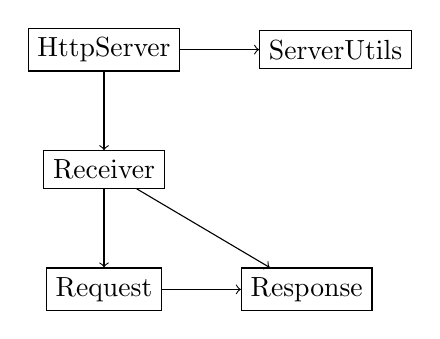
\begin{tikzpicture}
		\node[draw]	(HttpServer) {HttpServer};
		\node[draw, right=of HttpServer]	(ServerUtils) {ServerUtils};
		\node[draw, below=of HttpServer]	(Receiver) {Receiver};
		\node[draw, below=of Receiver]	(Request) {Request};
		\node[draw, right=of Request]	(Response) {Response};
		
		\graph {
			(HttpServer) -> (ServerUtils);
			(HttpServer) -> (Receiver) -> (Request) -> (Response);
			(Receiver) -> (Response);
		};
	\end{tikzpicture}
	\caption{模块关系图} \label{fig1}
\end{figure}
\section{系统实现}

\subsection{HttpServer}

\subsubsection{成员变量}

有成员变量serverSocket,为监听套接字。

\subsubsection{main()方法}

HttpServer.main()方法首先尝试调用ServerUtils.load(),初始化配置。这些配置通过ServerUtils相应Getter访问。

因为本程序没有GUI,所以通过ctrl+c来结束程序,因此需要捕获结束信号。HttpServer.main()接下来通过Runtime.getRuntime().addShutdownHook()来截获ctrl+c信号,当用户试图ctrl+c时,先打印出关闭服务器提示,接下来检查serverSocket的关闭状态,如果没有关闭就关闭它。注册完控制程序以后,打印关闭服务器的提示信息。

注册完关闭程序以后创建监听在ServerUtils中给出的地址的套接字,赋给serverSocket。然后在死循环里试图进行serverSocket.accept(),若无请求到达自然在阻塞状态,若有请求就根据请求的socket创建一个Receiver,新开一个线程执行Receiver.run()。

\section{系统测试与结果说明}

\section{其他需要说明的问题}

线程池。

\section{参考文献}
	
\end{document}

